\subsection{Silicon vertex tracker}
\label{sec:svt}

Achieving the best possible acceptance at low A$^\prime$ mass requires positioning the silicon as close as possible above and below the primary beam, where radiation and occupancy are both limiting factors.  As a result, the silicon must be actively cooled to retard radiation damage, hits must be read out quickly and tagged with the best possible time resolution to reduce effective occupancies, and the tracker must operate in a vacuum to eliminate beam-gas secondaries.  At the limit of feasibility from these considerations, the silicon in the first layer is only 0.5 mm from the center of the beam, so prudence dictates that the tracker be retractable from the beam. Meanwhile, achieving the best possible acceptance at high mass means that the active volume of the tracker fill as much of the magnet bore as possible.  Finally, both the mass and vertex resolution that determine the experimental sensitivity are dominated by multiple scattering effects, so minimizing material in the tracker is the principal design goal. A more complete discussion of the key requirements and design principles of the HPS Silicon Vertex Tracker (SVT) may be found in the initial proposal to the JLab PAC~\cite{HPS_PROP}.  

The HPS Test Run SVT, described and discussed in Chapter~\ref{sec:testrun2012}, achieved these goals with the minimal possible apparatus capable of delivering A$^\prime$ physics during a short run. Unlike the initial proposal for the full experiment, this design used a single type of silicon microstrip module with small stereo angle arranged into five layers and compromised redundancy, precision, and longevity in order to compress the project timeline and reduce the budget. In the process of developing this design, it was found that this simple system was capable of delivering a surprising fraction of the physics potential anticipated for the full experiment.  With this in mind, we now propose a design for the HPS SVT that builds upon the HPS Test SVT, principally by addressing the compromises made for HPS Test to ensure the best possible performance for A$^\prime$ physics within the envelope of the existing beam line layout and analyzing magnet.  This design uses the exact same sensors and readout chips, retaining the most successful elements of the HPS Test design and addressing the weaknesses identified during assembly and operation to ensure the success of the experiment.

\subsubsection{Layout}

The layout of the HPS SVT is summarized in Table~\ref{table:svt_layout} and shown in Figure~\ref{figure:svt_layout}. There are six measurement stations, or ``layers," placed immediately downstream of the target. Each layer comprises a pair of closely-spaced planes and each plane is responsible for measuring a single coordinate, or ``view''. Introduction of a stereo angle between the two planes of each layer enables three-dimensional tracking and vertexing.
%================
\begin{table}[h]
\begin{center}
\begin{tabular}{lcccccc}   
\hline \hline 
    Layer number & 1 & 2 & 3 & 4 & 5 & 6 \\      
\hline
    nominal $z$, from target (cm)  & 10 & 20 & 30 & 50 & 70  & 90 \\ 
    Stereo Angle (mrad)  & 100 & 100 & 100 & 50 & 50 & 50 \\ 
    Bend-plane resolution ($\mu m$)  & $\approx$60 & $\approx$60 & $\approx$60 & $\approx$120 & $\approx$120 & $\approx$120 \\ 
    Non-bend resolution ($\mu m$)  & $\approx$6 & $\approx$6 & $\approx$6 & $\approx$6 & $\approx$6  & $\approx$6 \\ 
    Number of sensors  & 4 & 4 & 4 & 8 & 8 & 8 \\ 
    Nominal dead zone in $y$ (mm)  & $\pm1.5$  & $\pm3.0$  & $\pm4.5$  & $\pm7.5$  & $\pm10.5$ & $\pm13.5$  \\ 
    Module power consumption (W) & 6.9 & 6.9 & 6.9 & 13.8 & 13.8 & 13.8 \\
\hline \hline
\end{tabular}
\caption[]{Layout of the HPS SVT.  The angle of stereo sensors is relative to the axial sensors that have their readout strips parallel to the edge of the dead zone.}
\label{table:svt_layout} 
\end{center}
\end{table}
%=================
\begin{figure}[ht]
    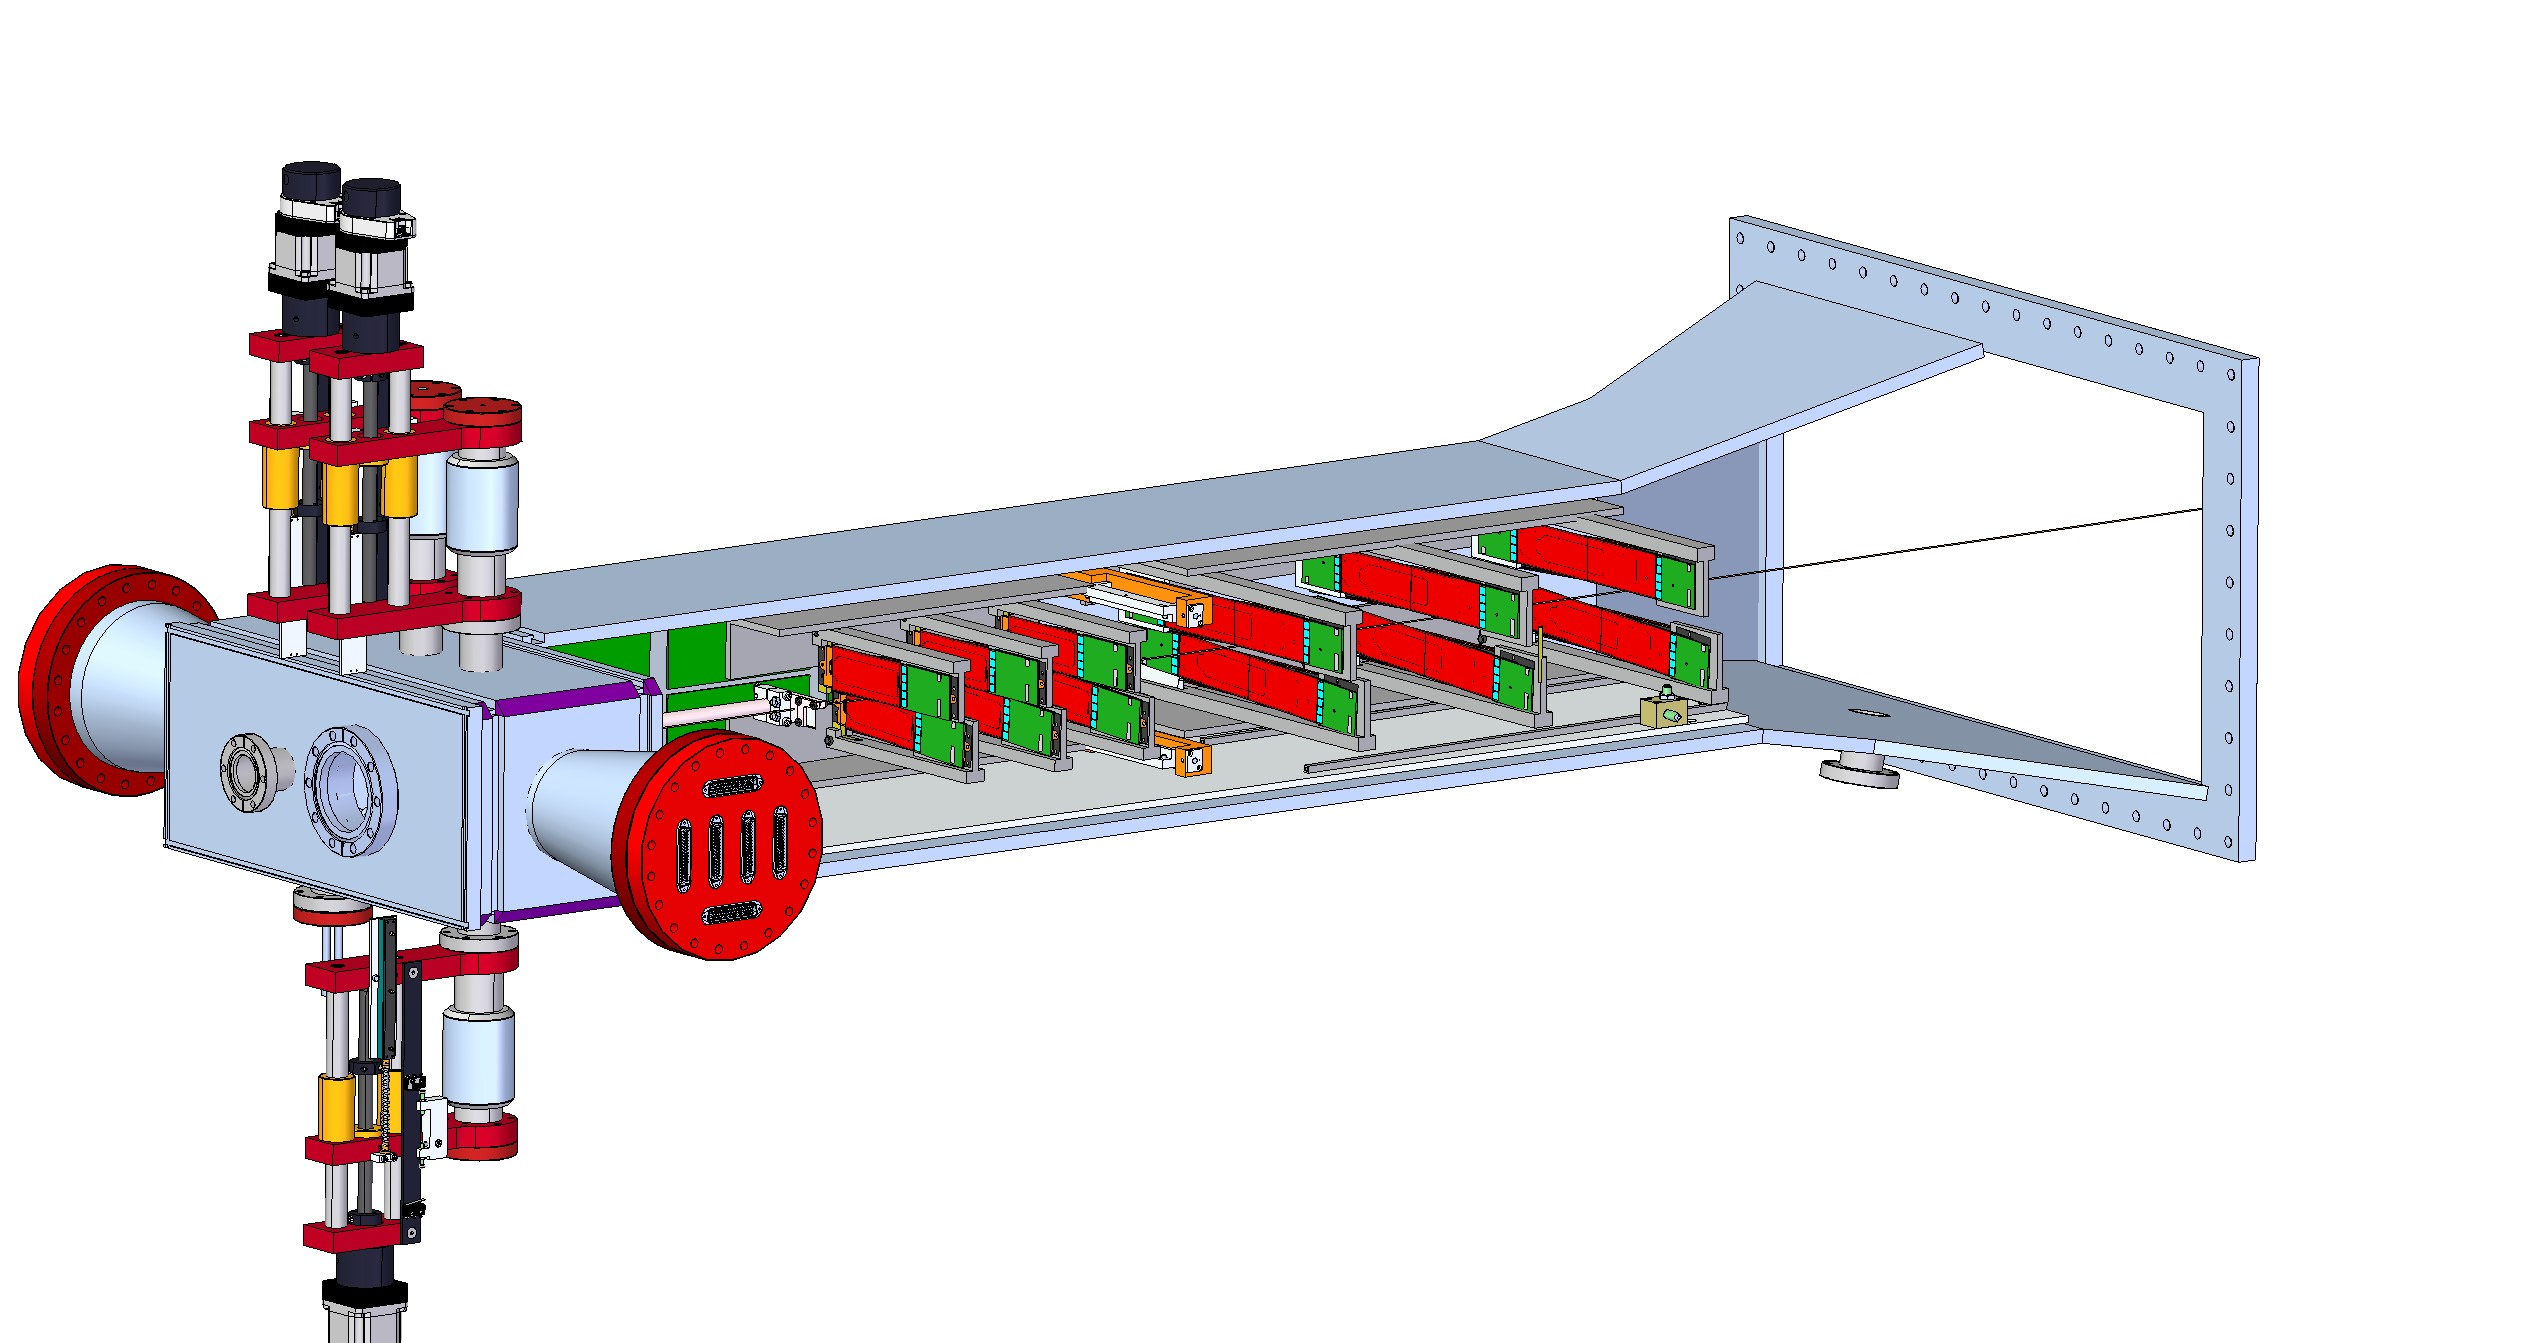
\includegraphics[width=\textwidth]{svt/figures/10dec6.jpg}
\caption{\small{A rendering of the concept for the HPS SVT.  The beam enters from the left through the vacuum box providing services to the SVT.  The silicon is shown in red and the hybrid readout boards in green.} }
\label{figure:svt_layout}
\end{figure}
%================

The layout of the first three layers is the same as in the HPS Test SVT, with a single sensor of coverage both above and below the beam and 100 milliradian stereo angle to balance acceptance against the resolution required for vertexing.  The last three layers are two sensors wide in the bend direction to better match the ECal acceptance and use 50 milliradian stereo, as in HPS Test, to break the tracking degeneracy that creates fake tracks from ghost hits in layers with the same stereo angle.  The first five layers cover the full acceptance of the ECal with one redundant layer.  The sixth layer has only slightly less acceptance than the ECal and results in an extra safety factor in tracking purity and improved momentum resolution for the vast majority of tracks.  Altogether, this layout comprises 36 sensors and 180 readout chips for a total of 23040 readout channels.

Acceptance for larger A$^\prime$ masses is limited by the size of the magnet but low-mass sensitivity depends on reconstructing tracks as close to the primary beam as possible; minimizing the so-called ``dead zone" surrounding the degraded primary beam in the mid-plane of the detector.  For the tracker, there are a number of considerations including proximity to beam halo and radiation damage in the first layer, ability to resolve time-overlapping hits, and the wall of pattern recognition errors at very high occupancies. With sensors capable of operation to $1.5 \times 10^{15}$ 1 MeV neq., readout with single-hit resolution of $\sim$2 ns and two-hit resolution of $\sim$50 ns, and pattern recognition robust to 2\% occupancy; the closest tolerable position of Layer 1 results in tracking acceptance outside of a 15 mrad dead zone around the beam plane.  In this configuration, the edge of the silicon in Layer 1 is 0.5 mm away from the center of the beam where occupancy from beam-gas curlers would be unacceptable. Therefore, along with the drive to minimize multiple scattering errors, the desire to maximize low-mass acceptance creates the principal design challenges for the SVT: a lightweight, movable, liquid-cooled tracker with superior time resolution and operated in vacuum.

\subsubsection{Module Design}

One strength of the HPS Test SVT is exceptionally low material budget, an average of 0.7\% $X_0$ per double-sided layer in the tracking volume with only 10\% of this from support material.  The HPS Test sensor modules achieve this figure by compromising the straightness, mechanical stability and cooling of the sensors.  The module design for HPS aims to maintain this material budget but eliminate these compromises by retaining the design of the carbon fiber half-modules but mounting them in a more robust way. Furthermore, this design allows the existing half-modules built for HPS Test to be reused for the first three layers of HPS, enabling the development of this module concept and the assembly of HPS to commence immediately and with a very small initial investment. 

A half module for the HPS Test SVT consists of a single microstrip sensor and a hybrid electronic readout board glued to a polyimide-laminated carbon fiber composite backing, as shown in Figure~\ref{fig:halfmodule_L1-3}.  
%=================
\begin{figure}[ht]
    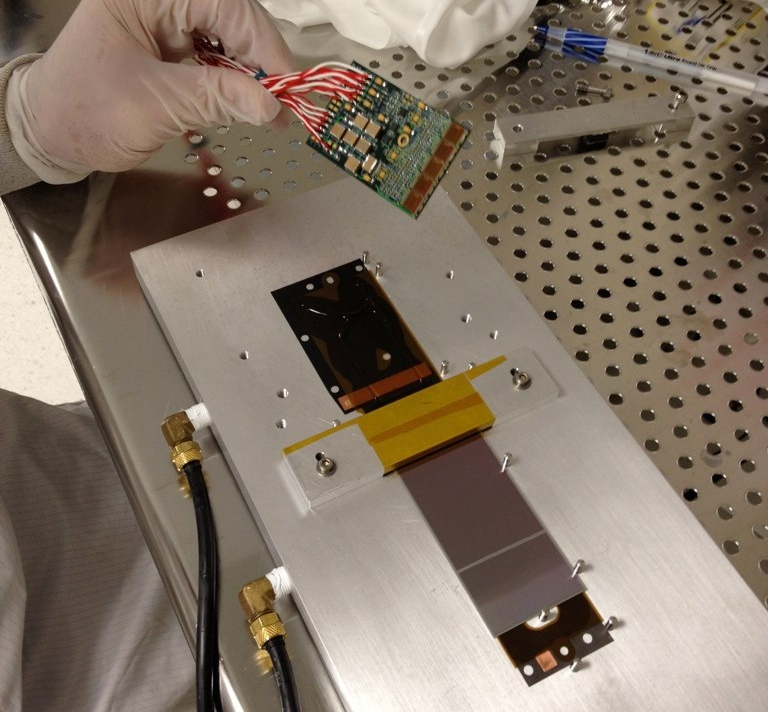
\includegraphics[width=4in]{svt/figures/half_module.jpg}
\caption{\small{A half module being assembled for Layers 1-3 of the HPS SVT. A silicon sensor and an APV25 readout hybrid are being glued to the Kapton laminated carbon fiber support frame.} }
\label{fig:halfmodule_L1-3}
\end{figure}
%================
A window is machined in the carbon fiber leaving only a frame around the periphery of the silicon to minimize material. A 50 $\mu$m sheet of polyimide is laminated to the surface of the carbon fiber with 1 mm overhang at all openings to ensure good isolation between the back side of the sensor, carrying high-voltage bias, and the carbon fiber which is held near ground.  The sensors are single-sided, radiation tolerant, p$^+$ in n bulk, AC coupled, poly-biased sensors fabricated on $<$100$>$ silicon manufactured by the Hamamatsu Photonics Corporation for the RunIIb upgrade of the D\O\ silicon detector. The sensors have 60(30) $\mu$m readout(sense) pitch and are read out by APV25 chips operating in multi-peak mode, allowing single hit position resolution of $\sim$6 $\mu$m and tagging of individual hit times with a precision of approximately 2 ns.  Although specified to achieve 350 V bias, approximately 90\% of sensors break down above 1000 V, sufficient to operate layer one of the SVT with full efficiency for six months at full beam intensity.

For HPS Test, the half-modules were sandwiched back-to-back around an aluminum cooling block at the hybrid end and a similar PEEK spacer block at the other.  To allow for module rework, the modules were assembled with hardware and thermal compound instead of adhesive and have no stiffening material between the two sensors. For simplicity, only the cooling block at the hybrid end is supported, resulting in deviations in the planarity of the sensors as large as a few hundred microns at the cantilevered end. Furthermore, the lack of cooling at the unsupported end where there is no heat source from readout electronics limits the temperature achievable at the most highly irradiated portion of the sensor, a very small spot along the edge of the sensor adjacent to the dead zone.  Improved cooling is necessary to achieve the longevity required for the longer running time envisioned for the HPS detector.

For layers 1-3 of HPS, these same half-module structures will be tensioned, like bicycle spokes, between a pair of cooling blocks held by a grooved aluminum base, as shown in Figure~\ref{fig:newmodule_L1-3}. 
%=================
\begin{figure}[ht]
    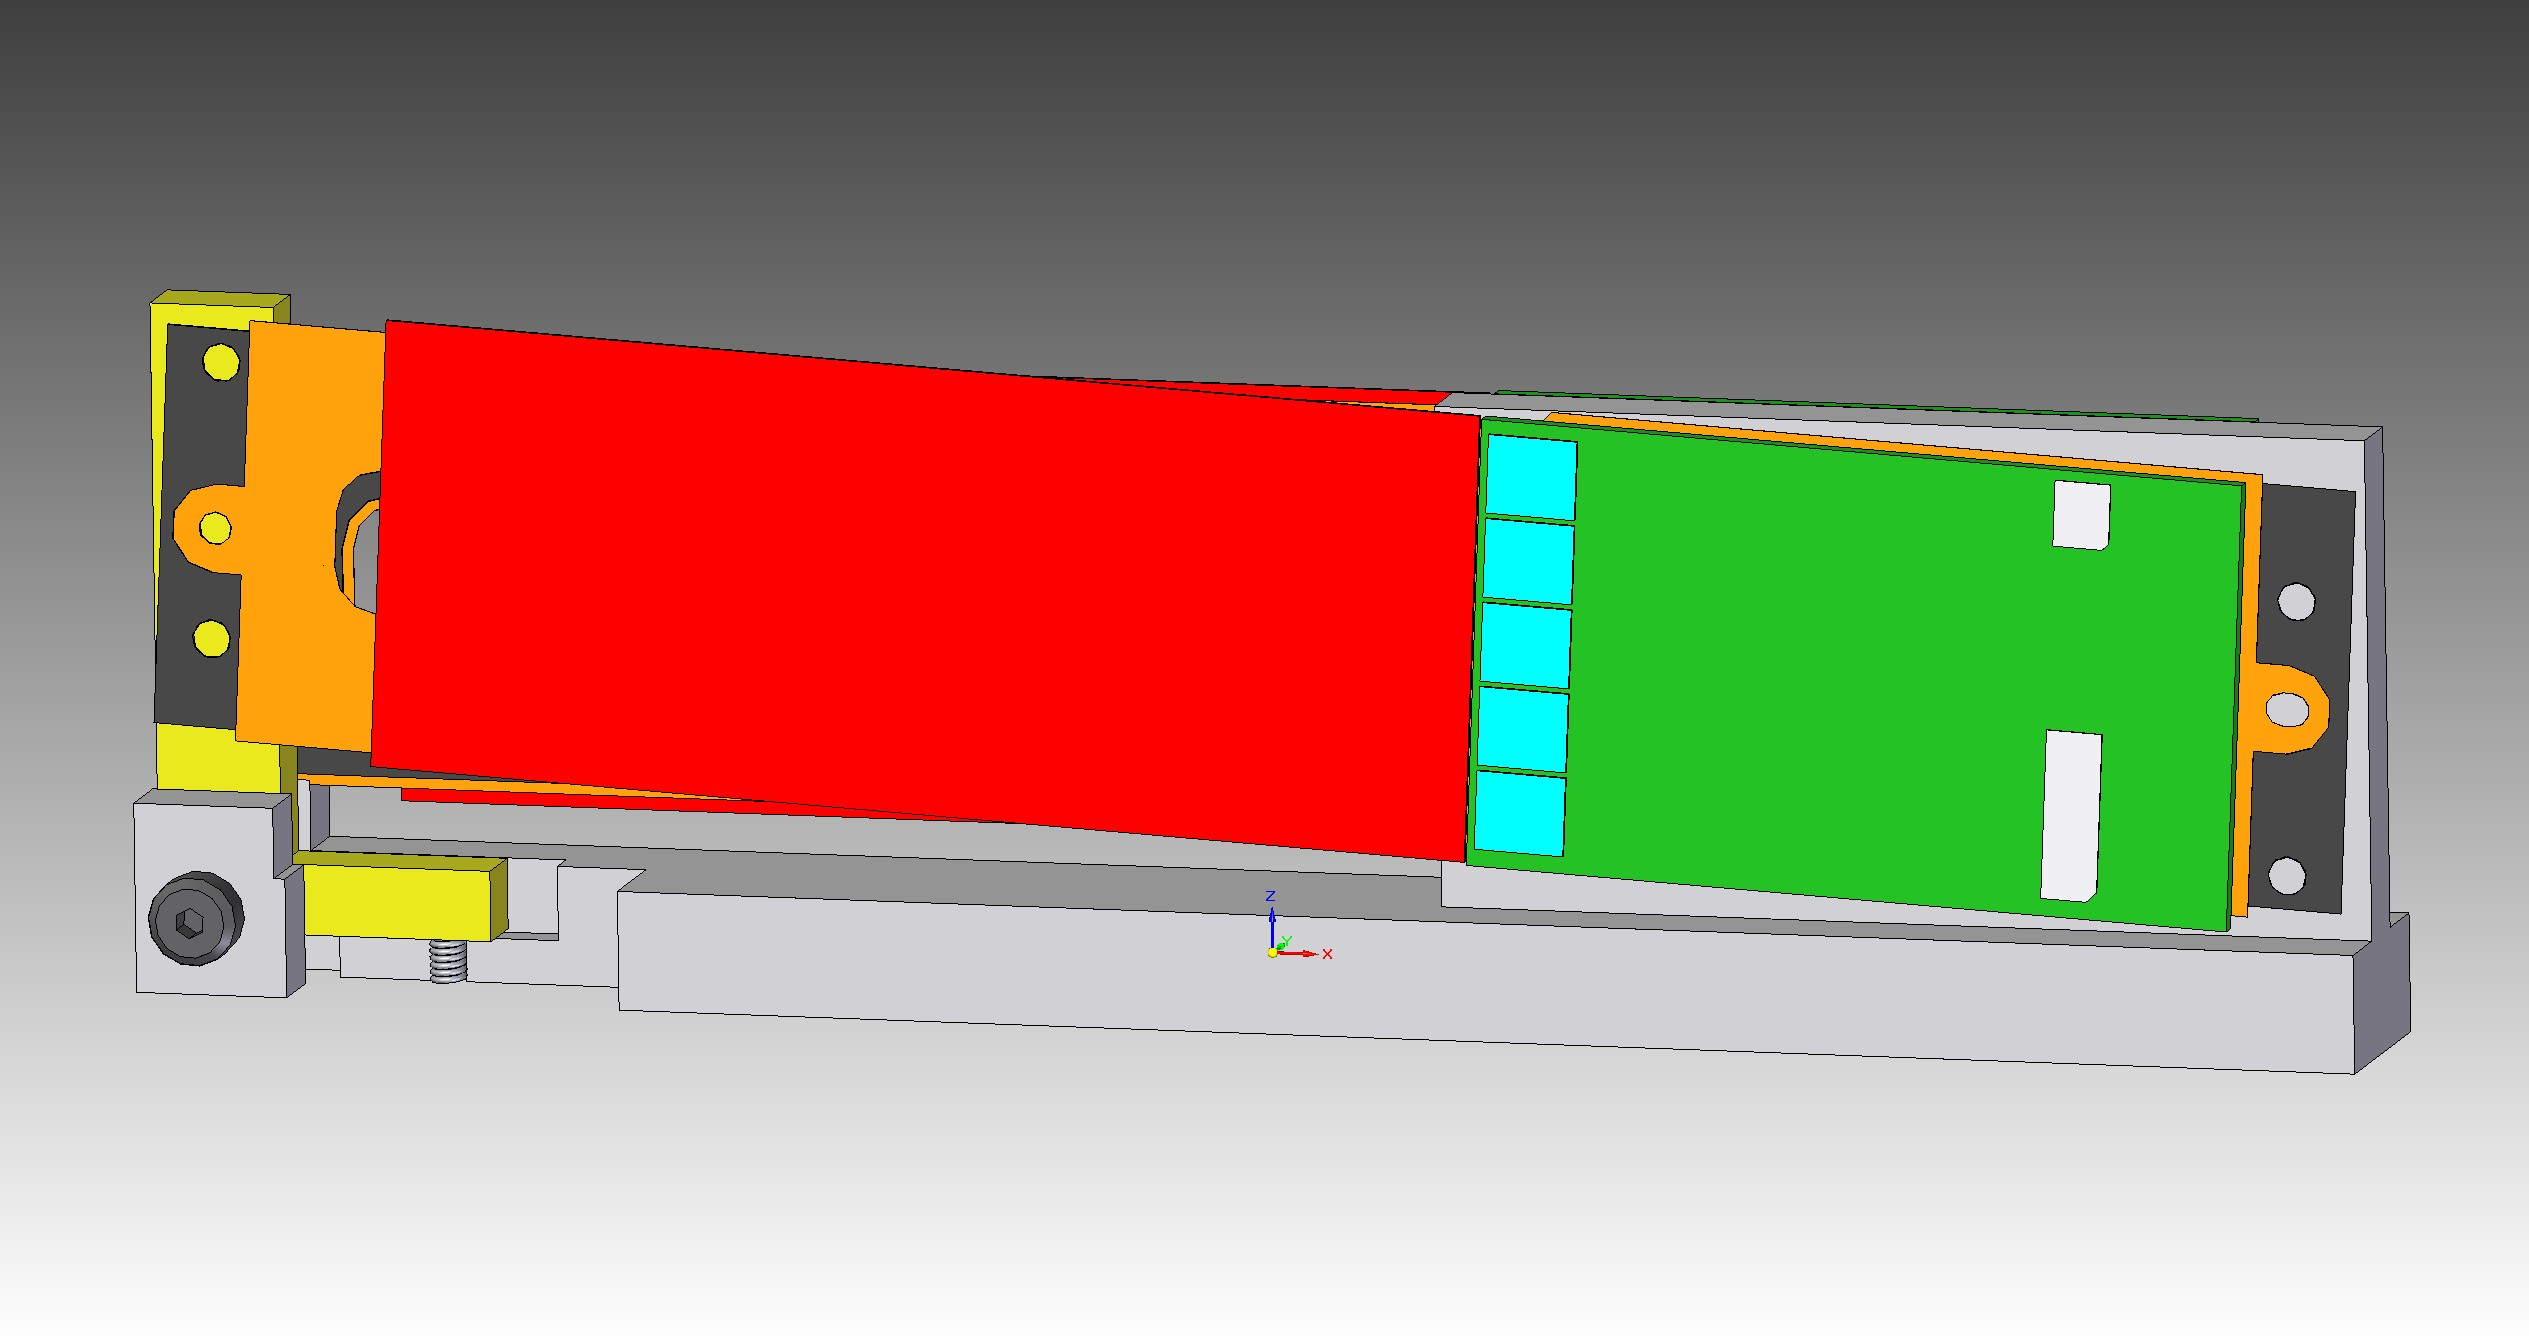
\includegraphics[width=\textwidth]{svt/figures/10dec3.jpg}
\caption{\small{A rendering of the concept for the new modules for Layers 1-3 of the HPS SVT.  A cutaway at the left shows the spring and lever mechanism that maintains tension on the carbon fiber of the half modules.} }
\label{fig:newmodule_L1-3}
\end{figure}
%================
Rather than building manifolds to provide cooling to these blocks and attempt to isolate them thermally from the underlying support structure as in HPS Test, the entire aluminum support structure will be cooled.  The block at the hybrid end of the module is fixed, while the other pivots on a shoulder screw with a small stainless compression spring providing tension of approximately 40 N and taking up the 60 micron differential contraction between the half module and the support structure during a 30 $^\circ$C cool down. The same low-viscosity thermal compound used in HPS Test will provide the thermal contact in the pivot joint between the grooved base and the pivoting block and generates a negligible temperature drop across the gap. This arrangement results in much flatter silicon, much better mechanical stability and much better cooling that provided by the previous design for layers 1-3. With temperature stability during running better than 1 $^\circ$C, dimensional stability of the tracker will be better than intrinsic measurement resolutions and more than an order of magnitude better than the resolution limitation from multiple scattering effects.

More importantly, this scheme allows the ultra-thin design to be extended to the longer, double-sensor half-modules of layers 4-6 that have a pair of silicon sensors in the middle and a readout hybrid at each end, as shown in Figure~\ref{fig:newmodule_L4-6}.  
%=================
\begin{figure}[ht]
    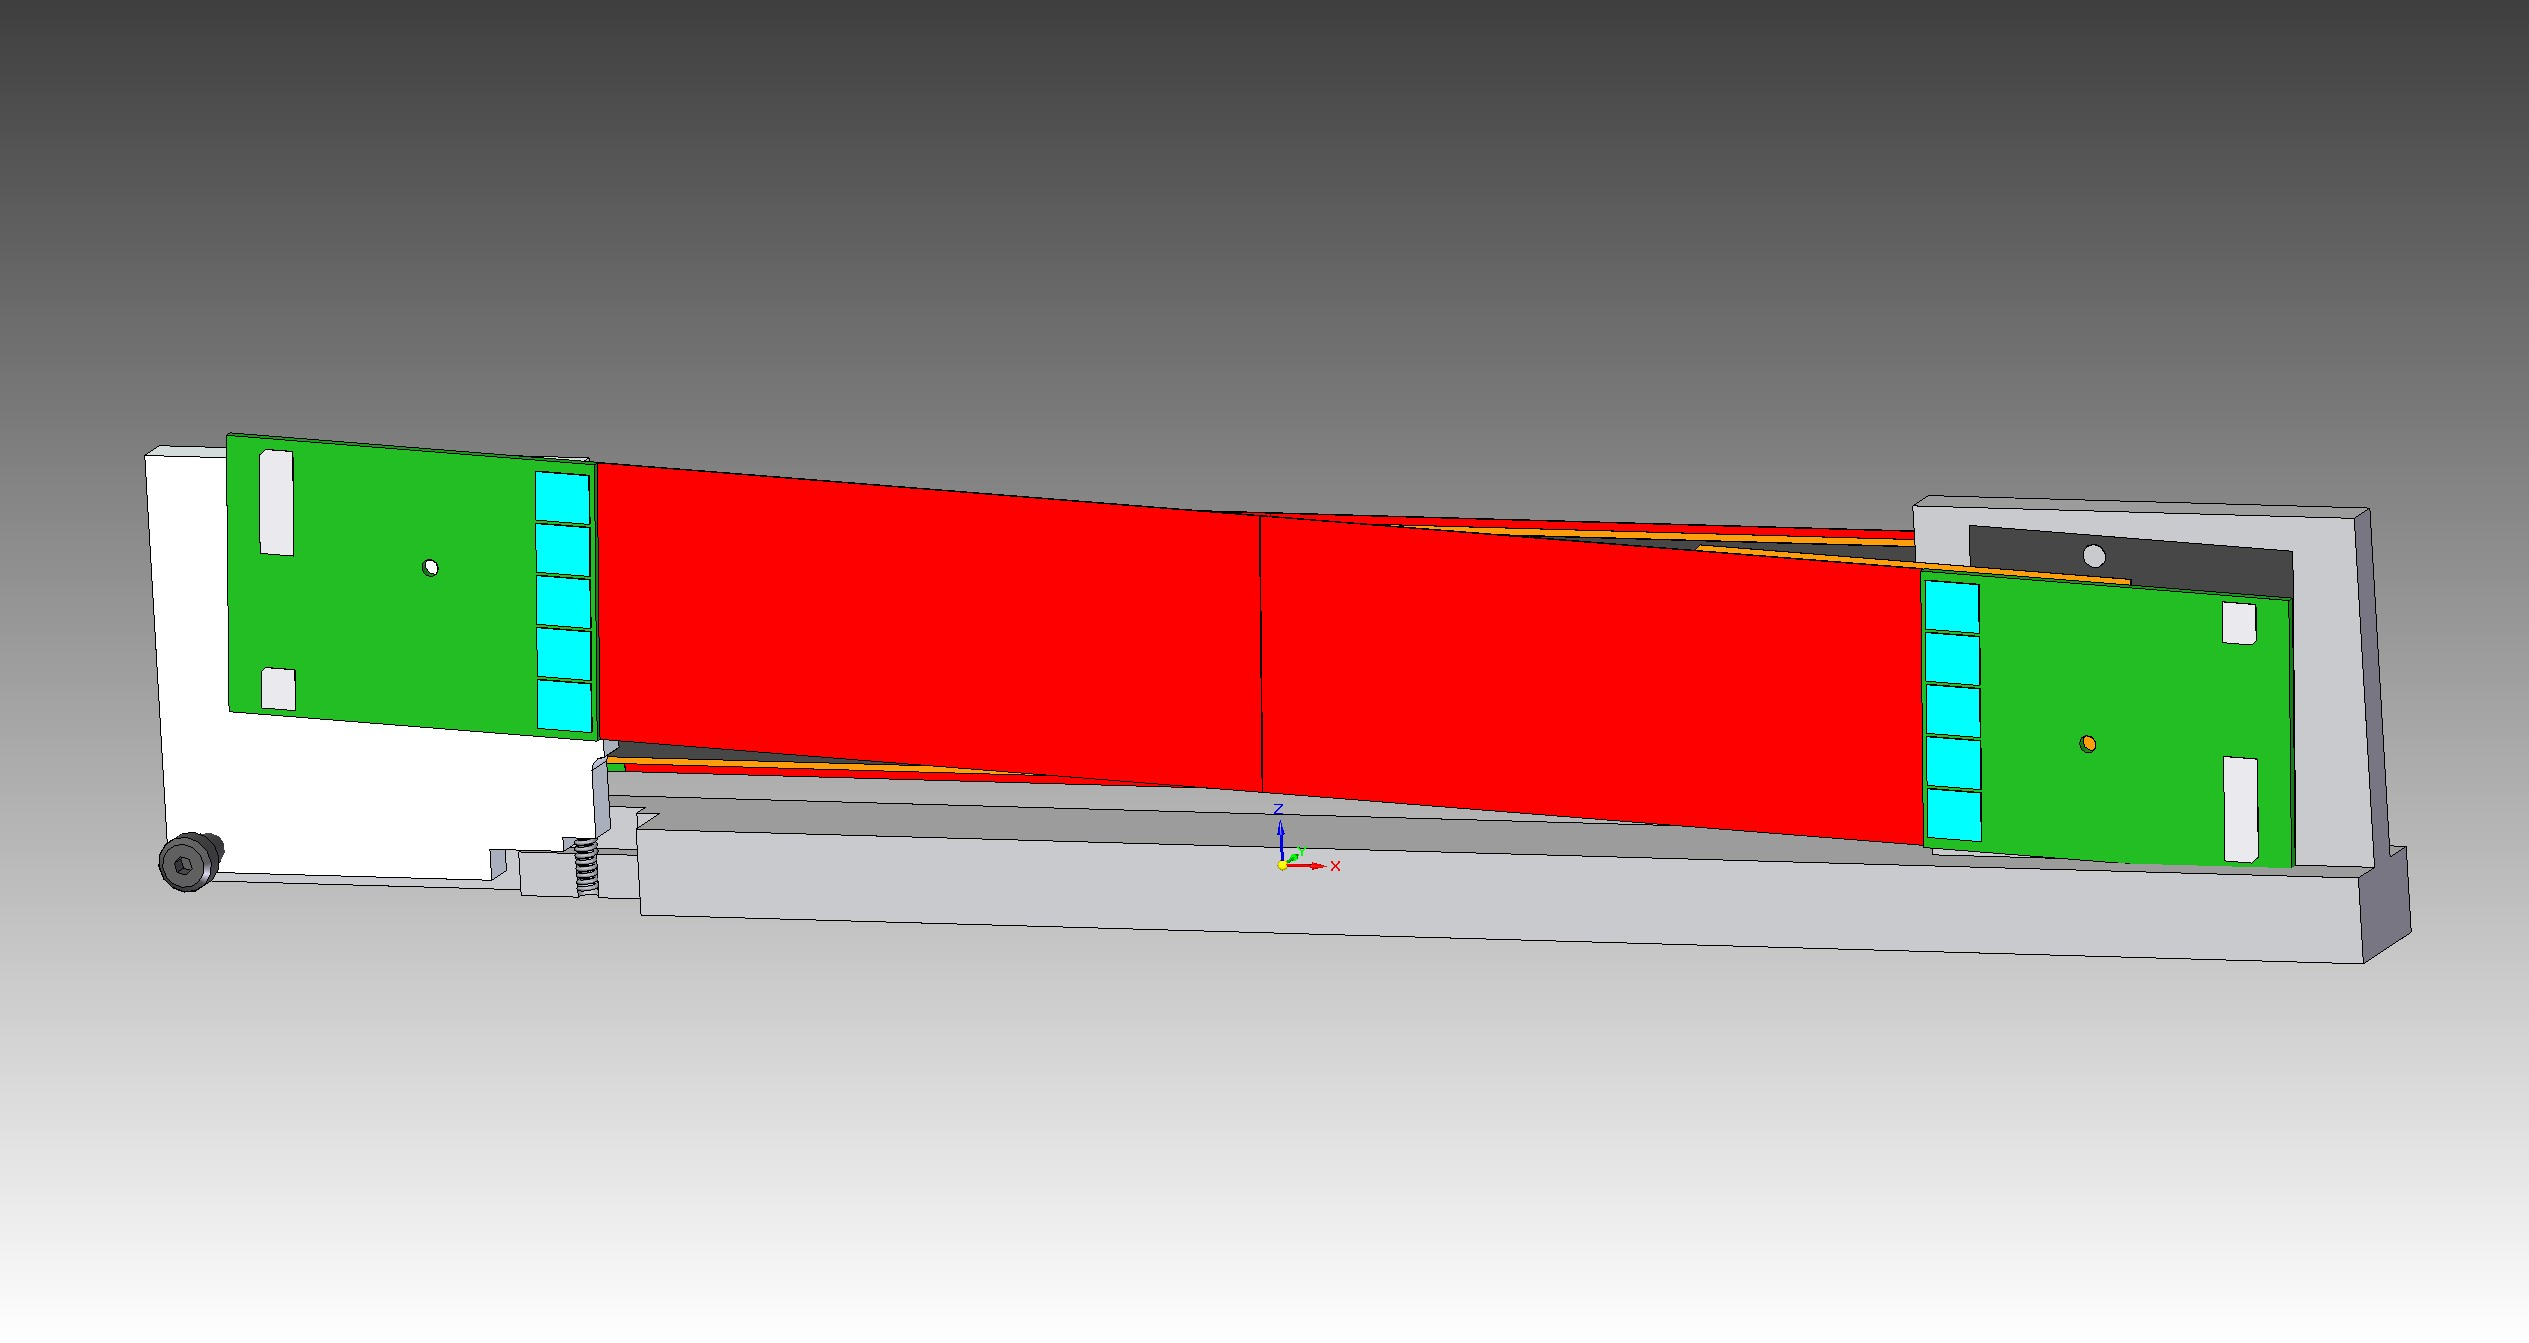
\includegraphics[width=\textwidth]{svt/figures/10dec1}
\caption{\small{A rendering of the concept for the new modules for Layers 4-6 of the HPS SVT.  A cutaway at the left shows the mechanism responsible for keeping the half modules under tension.} }
\label{fig:newmodule_L4-6}
\end{figure}
%================
With a larger heat load to transmit, the temperature drop through the pivot joint of the moving block will be approximately 0.5 $^\circ$C. To accommodate the length of these double modules across the width of the vacuum chamber, the hybrids will be shortened by approximately 20\%.  Through the use of polyimide flex cables instead of twisted pair and the elimination of superfluous circuitry, this footprint can be achieved with little effort.  Aside from this, only minor changes to the conceptual design of the half module concept of HPS Test are envisioned to reduce assembly effort.

\subsubsection{Mechanical Support, Cooling and Services}

Sag of the aluminum support plates, when subjected to the bending load of the long motion levers, was the largest source of mechanical imprecision in the HPS Test SVT.  For HPS, this motion system will be reused but with changes to eliminate this weakness. First, only layers 1-3 will retract, reducing the length of the support plate by a factor of two.  Replacing the twisted pair readout with flex cables eliminates the largest external load on the plate.  Finally, the 0.5 inch plate will be replaced by a 0.25 inch plate with 0.25 inch sides, forming a u-channel for increased stiffness, as shown in Figure~\ref{fig:newsupport}. 
%=================
\begin{figure}[ht]
    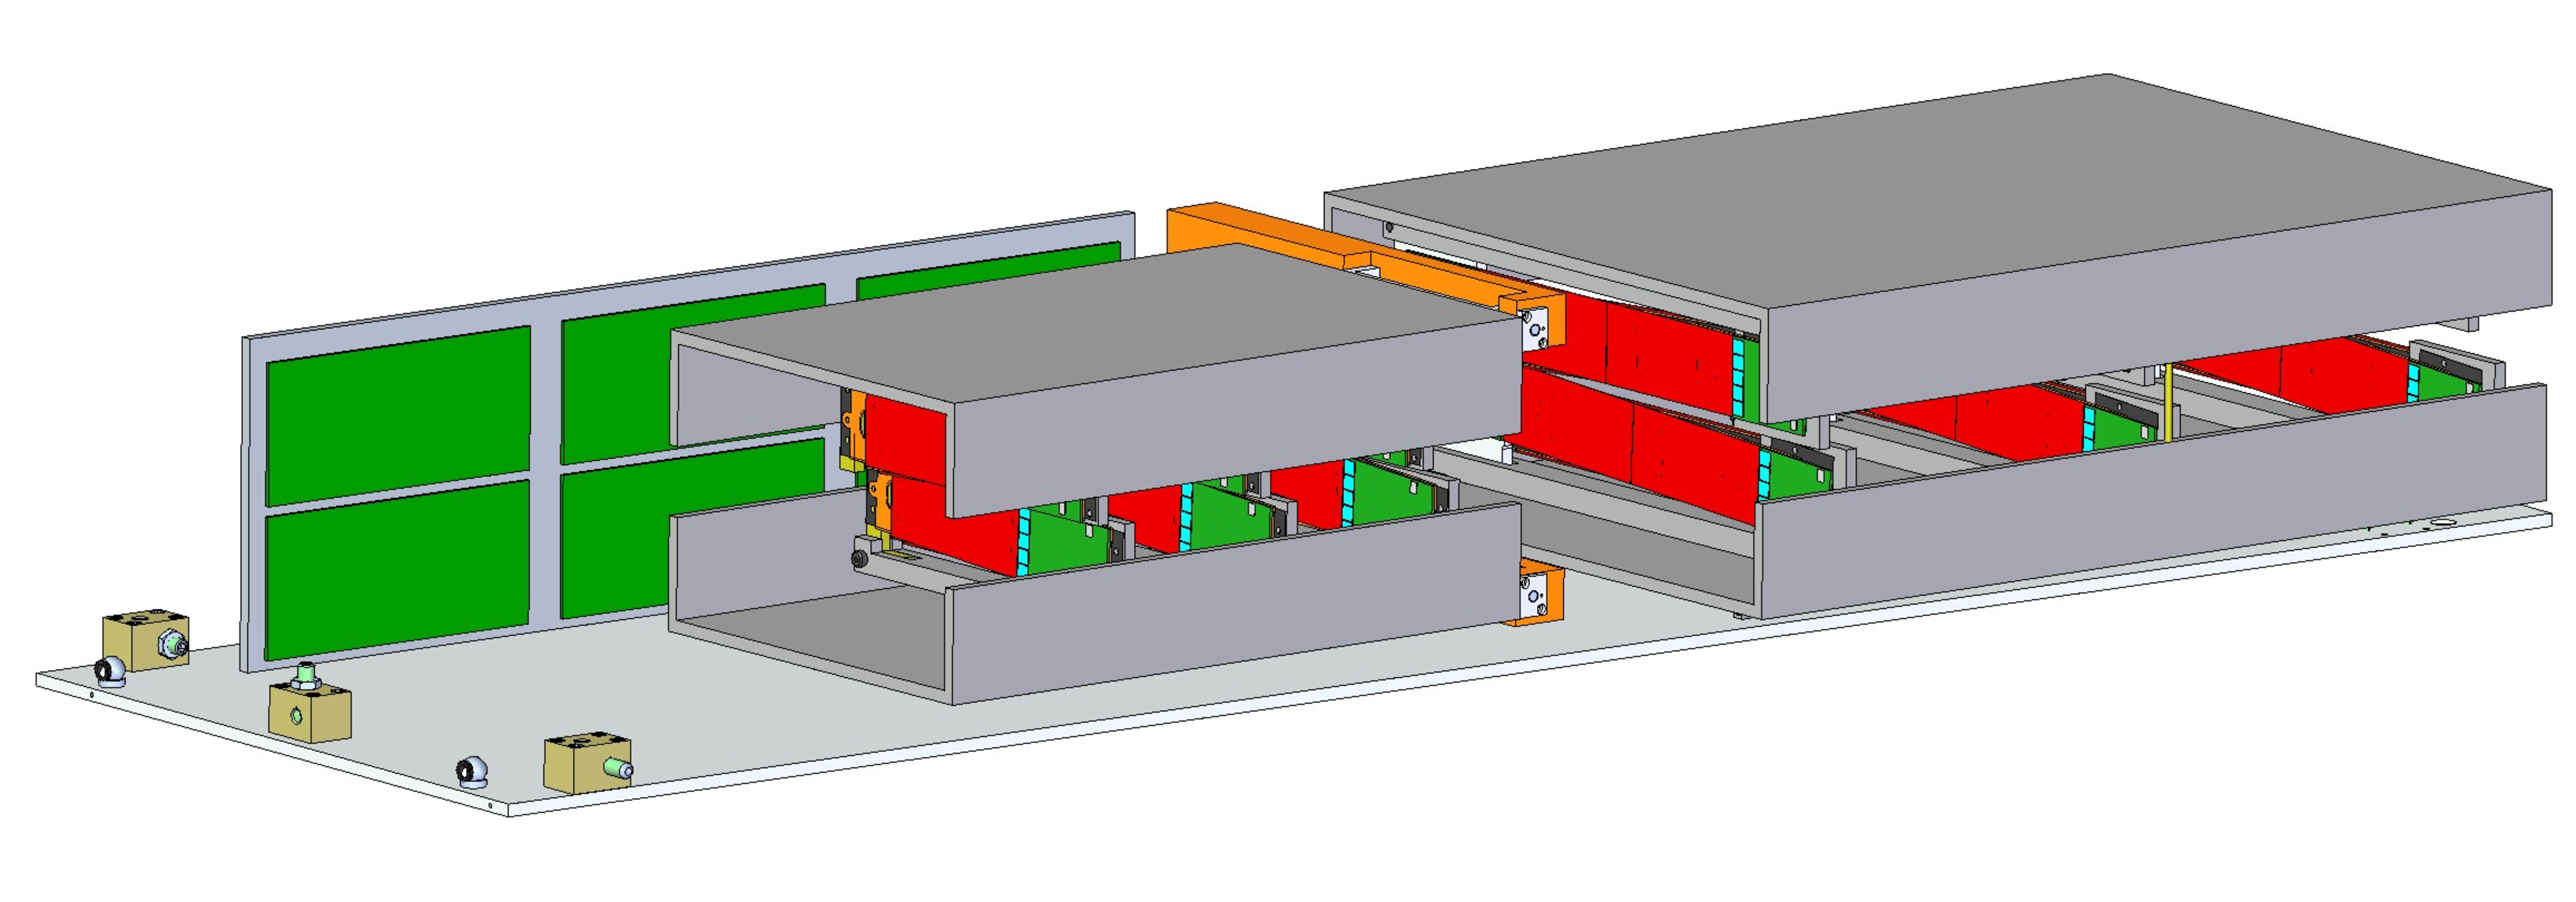
\includegraphics[width=\textwidth]{svt/figures/10dec8}
\caption{\small{A rendering of the support concept the HPS SVT.  The modules are mounted in cooled channels.  The channels for Layers 1-3 pivot on a downstream "C-support" and are moved by lever extending upstream to linear shifts on the vacuum box, as in HPS Test.  Layers 4-6 are fixed in place. The DAQ boards, shown in green, are mounted to a separate cooling plate located in a low-neutron region upstream on the positron side of the detector.} }
\label{fig:newsupport}
\end{figure}
%================
The walls of this support channel will extend almost to the dead zone and the entire structure will be cooled by large, embedded copper tubes. Surrounding the modules over most of the solid angle, these support channels will nearly eliminate thermal radiation from the walls of the vacuum chamber, the primary heat load on the sensors.  Layers 4-6 will be mounted inside similar cooled channels but will be fixed since they are already far enough from the dead zone for safety during beam tuning. These two support structures will be mounted to a single baseplate as before, with complete adjustability relative to the vacuum chamber.  

Readout and power for HPS Test required 30 conductors per hybrid, or a total of 600 lines, with even that count requiring elimination of sense for DVDD on the hybrids.  It does not appear feasible to scale this solution by nearly a factor of two for HPS.  Instead, we plan to provide digitization and optical readout of the APV25 data as well as shared power for the hybrids on boards placed inside the vacuum chamber, as described in Section~\ref{sec:svt_daq}.  In consideration of the DAQ requirements and the environment inside of the vacuum chamber, it appears that there is a natural location for support and cooling of the necessary boards adjacent to layers 1-3 on the positron side.  This structure consists of a single vertically-oriented plate with an embedded cooling loop, shown in Figure~\ref{fig:newsupport}. By separating the readout boards on the outside of this plate by the same 20 cm separation of layers 4-6, a single cable solution can be employed to connect the hybrids of layers 4-6 to these boards.  This leaves layers 1-3 equidistant from the pair of readout boards on the inner side, where a second cable type can connect to the existing pigtail connectors for those hybrids.  The feedthroughs required for power and data in this design fit easily on one of the two flanges in the existing vacuum box, leaving the other flange for additional cooling, eliminating the need for a cooling manifold inside of the vacuum chamber.
